\documentclass[aspectratio=1610]{beamer}
%\documentclass[aspectratio=1610,handout]{beamer}

% Common packages

\usepackage[english]{babel}
\usepackage[latin1]{inputenc}
\usepackage{times}
\usepackage{hyperref}
\usepackage[T1]{fontenc}
\usepackage{multicol}
\usepackage{ifthen}
\usepackage{subfigure}
\usepackage{color}

% Common settings for all lectures in this course

% Beamer version theme settings

\usetheme[hideothersubsections,width=0cm]{Goettingen}
\usecolortheme{sidebartab}

%\usefonttheme[only large]{structurebold}

%\setbeamercolor{sidebar right}{bg=black!15}

\setbeamerfont{title}{series=\normalfont,size=\LARGE}
\setbeamerfont{title in sidebar}{series=\bfseries}
\setbeamerfont{author in sidebar}{series=\bfseries}
%\setbeamerfont*{item}{series=}
%\setbeamerfont{frametitle}{size=}
%\setbeamerfont{block title}{size=\small}
%\setbeamerfont{subtitle}{size=\normalsize,series=\normalfont}

\setbeamertemplate{navigation symbols}{}


%\setbeamertemplate{itemize subitem}[square]
%\setbeamercolor{itemize subitem}{fg=red!100}
%\setbeamertemplate{itemize subsubitem}[circle]

% the beginning of each subsection:
%\AtBeginSubsection[]
%{
%  \begin{frame}<beamer>{Outline}
%    \tableofcontents[currentsection,currentsubsection]
%  \end{frame}
%}

%\beamerdefaultoverlayspecification{<+->}

\setlength{\fboxrule}{1pt}
\newcounter{Timestamps}
%\setcounter{Timestamps}{1}

\newcommand{\timestamp}[1] {\ifthenelse{\value{Timestamps} =
    1}{\alert{(#1 min)}}{}}
\newcommand{\reference}[1]{{\hfill \tiny \textcolor{gray}{#1}}}

\newcommand{\mweak}{m_W}
\newcommand{\mgut}{m_{\text{GUT}}}
\newcommand{\gev}{\text{GeV}}
\newcommand{\tev}{\text{TeV}}
\newcommand{\phiCP}{\phi_{\text{CP}}}
\newcommand{\mhu}{m_{H_u}}
\newcommand{\mhd}{m_{H_d}}
\newcommand{\mtl}{m_{Q_3}}
\newcommand{\mtr}{m_{\bar{U}_3}}
\newcommand{\at}{A_t}
\newcommand{\atgut}{\at (\mgut)}
\newcommand{\atweak}{\at (\mweak)}
\newcommand{\atsqgut}{\at^2 (\mgut)}
\newcommand{\atsqweak}{\at^2 (\mweak)}
\newcommand{\ab}{A_b}
\newcommand{\cmax}{c_{\text{max}}}
\newcommand{\mmix}{\mathcal{A}_{\tilde{t}}}

\definecolor{gold}{RGB}{200, 150, 0}

\title{Content Modeling of Tweets on Twitter}

\author{David Sanford}

\institute{Data Science Immersive\\ General Assembly}

\date{Thursday March 9, 2017}


\begin{document}

\begin{frame}
  \titlepage
\end{frame}

%%%%%%%%%%%%%%%%%%%%%%%%%%%%%%%%%%%%%%%%%%%%%%%%%%%%%%%%%%%%%%%%%%%%%%%%%%%%%%%%

\begin{frame}{Enter the Cacophony}

  \begin{itemize}
  \item<alert@1> Twitter contains an enormous amount of data
  \item<2-|alert@2> But the breadth of topics makes an unfiltered
    stream meaningless noise
  \end{itemize}

  
  \begin{center}
    \uncover<3->{ \textcolor{blue}{How can tweets related to a
        particular subject be tagged?} }
  \end{center}

  \uncover<4-> {
    \begin{itemize}
    \item Keyword/user/location filtering can reduce the stream
      somewhat
      \begin{itemize}
      \item Requires meaningfully restrictive keywords
      \item Useful for sample sets, but will cut away a large amount
        of useful data
      \end{itemize}
    \item Many subject-related tweets will not contain keywords
    \item Some keywords have more general context than desired
    \end{itemize}
  }

  \begin{center}
    \uncover<5->{ \textcolor{green}{\bf Is there a better way?} }
  \end{center}

\end{frame}

%%%%%%%%%%%%%%%%%%%%%%%%%%%%%%%%%%%%%%%%%%%%%%%%%%%%%%%%%%%%%%%%%%%%%%%%%%%%%%%%

\begin{frame}{Going Beyond Simple Tagging}
  \begin{center}
    \textcolor{violet}{\bf Tweet content beyond keywords may
      indicated subject relevance}
  \end{center}

  \uncover<2->{
    \begin{itemize}
    \item Able to select around mis-spellings and abbreviations
    \item Captures related words and/or terminology beyond the scope
      of keyword searches
      \begin{itemize}
      \item Techinical terms related to a subject
      \item Unique terms in various types of fiction
      \item Terms more prevalent in a subject
      \end{itemize}
    \item Captures sets of relevant and/or iconic words
    \end{itemize}
  }

  \uncover<3->{
    \begin{center}
      \textcolor{orange}{\bf NLP and Machine Learning can attempt to
        identify these features}
    \end{center}
  }

\end{frame}

\begin{frame}{Project Goals}
  \begin{itemize}
    \item Identify a topic and tweet collection methodology which
      produces a sufficiently clean sample
    \item Identify the best modeling methodology
    \item Clean tweets
    \item Perform binary classification of topic-related tweets
      against an unfiltered stream of tweets
    \item Cluster tweets aggregated on keywords to identify genres
      within the topics
  \end{itemize}

\end{frame}


\begin{frame}{Choosing the Right Data Set}
  \begin{center}
    \textcolor{red}{\bf As a test of concept, a clean data set of
      subject-related tweets must be used}
  \end{center}

  \uncover<2->{
    \begin{center}
      \textcolor{blue}{Tweets from a curated set of users may be usable}
    \end{center}
    \begin{itemize}
    \item Requires a large number of users and careful curation
    \end{itemize}
  }

  \uncover<3->{
    \begin{center}
      \textcolor{green}{A keyword search can get a larger number of
        tweets covering from many users}
    \end{center}
    \begin{itemize}
    \item Requires careful choice of keywords
    \end{itemize}

    \hspace*{-0.75cm}
    \begin{tabular}{|p{3.5cm}|p{6cm}|p{4.5cm}|}
      \hline
      \textbf{Topic} & \textbf{Good Keywords} & \textbf{Bad Keywords} \\
      \hline
      Academic Subject & \_\_\_\_ Studies, \_\_\_\_ Sciences &
      Business, Economics \\
      \hline
      Tabletop RPG & Dungeons \& Dragons, Shadowrun & Werewolf, Call
      of Cthulhu \\
      \hline
      Tabletop Games & Settlers of Catan, Scrabble & Risk, Dominion \\
      \hline
      Video Games & Mario, Zelda, Tetris, Angry Birds & Civilization,
      Battlefield \\
      \hline
    \end{tabular}
  }


\end{frame}

\begin{frame}{It's a me!  Mario! -- And Friends}
  \begin{center}
    \textcolor{green}{\bf Of the topics I considered, video games had
      the greatest number of unique names}
  \end{center}

  \begin{itemize}
  \item https://en.wikipedia.org/wiki/List\_of\_best-selling\_video\_games
  \item https://en.wikipedia.org/wiki/List\_of\_video\_games\_considered\_the\_best
  \end{itemize}
  
  
{\tiny \textbf{Accepted Keywords:} Zelda, Tetris, Mario, Chrono
  Trigger, Street Fighter, Final Fantasy, Metroid, Half-Life, Resident
  Evil, Metal Gear, Castlevania, Pokemon, BioShock, SoulCalibur,
  StarCraft, Shadow of the Colossus, Doom, Diablo, World of Warcraft,
  Donkey Kong, Pac-Man, Halo, Deus Ex, Space Invaders, Sonic,
  Counter-Strike, Grim Fandango, Portal, Mass Effect, Last of Us, Star
  Fox, Mega Man, EarthBound, Prince of Persia, Call of Duty, Dark
  Souls, Perfect Dark, Ico, The Elder Scrolls, Skyrim, Morrowind,
  Silent Hill, Shenmue, Grand Theft Auto, Okami, Double Dragon, Red
  Dead, Galaga, Tomb Raider, Fallout, Uncharted, Assassin's Creed,
  Minecraft, Kingdom Hearts, Xenogears, Overwatch, Wii Sports, Wii
  Fit, The Sims, Terraria, Brain Age, Need for Speed, Lemmings, Madden
  NFL, Star Wars: Battlefront, Tom Clancy's, Duck Hunt, Splatoon,
  Super Smash, Dynasty Warriors, Monster Hunter, Kirby, Fire Emblem,
  Animal Crossing, God of War, Tekken, Garry's Mod, Myst, Angry Birds,
  Candy Crush, Fruit Ninja, Block Breaker, Doodle Jump, Space
  Invaders, Galaxian, Mortal Combat, Pong, Crysis}

{\tiny \textbf{Examples of Rejected Keywords:} Civilization,
  Battlefield, Asteriods, Fable, Journey}

\end{frame}


\begin{frame}{NLP Modeling for Tweets}
  \begin{center}
    \textcolor{teal}{\bf Only bag-of-words style models with
      transformations are likely to be relevant to tweets}
  \end{center}

  \uncover<2->{

    \begin{multicols}{2}
      \begin{itemize}
      \item Tweets often lack sentence structure
      \item Mis-spellings and abbreviations are common
      \item Many different levels and styles of grammar are on display
      \item Emojis and hashtags used in place of words
      \item Many tweets are ``stubs''
      \item Large number of documents in corpus makes tfidf useful
      \end{itemize}
 


      \begin{tabular}{|p{6cm}|}
        \hline
        {\small Zelda's super neat but I've experienced more severe
          frame drops in the first 5 minutes then I'd like to} \\
        \hline
        {\small How To Spot The Difference Between Battleborn And
          Overwatch \#Overwatch \#Overwatch https://t.co/Xj8ryeq5Tz
          https://t.co/uRCxip2kaR} \\
        \hline
        {\small RT @ForceComYT: \#Overwatch - Deutsch / German Let's
          Play - S03 - \#Competitive Placement Match \#07 -
          https://t.co/PVp3YzYQBf \#LetsPlay} \\
        \hline
      \end{tabular}
    \end{multicols}
  }

\end{frame}



\begin{frame}{Tweet-Cleaning}
  \begin{center}
    \textbf{Tweets are messy! Significant amounts of cleaning
      is required.}
  \end{center}

  \begin{multicols}{2}
    \begin{itemize}
    \item \only<1>{Retweet references}
      \only<2->{\textcolor{red}{Retweet references}}
    \item \only<1>{ Hashtags} \only<2->{\textcolor{green}{Hashtags}}
    \item User references
    \item Emojis
    \item \only<1>{Links} \only<2->{\textcolor{blue}{Links}}
    \item \only<1>{Keywords} \only<2->{\textcolor{violet}{Keywords}}
    \item Proper names
    \item \only<1>{Unintelligible strings}
      \only<2->{\textcolor{gold}{Unintelligible strings}}
    \end{itemize}
  \end{multicols}
 
  \uncover<2->{
    \begin{center}
      \textbf{As a first pass, I treat all the above items as ``stop
        words'' and remove them.}
    \end{center}

    \begin{tabular}{|p{6cm}|p{6cm}|}
      \hline {\small \textcolor{violet}{Zelda}'s super neat but I've
        experienced more severe frame drops in the first 5 minutes then
        I'd like to} & {\small 's super neat but i've experienced more
        severe frame drops in the first 5 minutes then i'd like to} \\
    
      \hline {\small \textcolor{red}{RT @ForceComYT:}
        \textcolor{green}{\#Overwatch} - Deutsch / German Let's Play -
        \textcolor{gold}{S03} - \textcolor{green}{\#Competitive} Placement
        Match \textcolor{green}{\#07} -
        \textcolor{blue}{https://t.co/PVp3YzYQBf}
        \textcolor{green}{\#LetsPlay}} & {\small - deutsch / german let's play
        - - placement match -} \\ \hline
    \end{tabular}
  }

\end{frame}



\begin{frame}{NLP Processing -- Warped Tweets}
  \begin{center}
    \textcolor{blue}{Initial Data Set -- 10K tweets from video game
      and unfiltered streams for both  training and validation sets}
  \end{center}

  \begin{multicols}{2}
  \begin{itemize}
  \item Training set used to train tf-idf vectorized model
    \begin{itemize}
    \item min\_df= 0.001, max\_df=0.5
    \item Stop words left in
    \item 1172 words kept
    \end{itemize}
  \item Tf-idf vectors passed through truncated svd
    \begin{itemize}
    \item 200 Components kept
    \item Explains 56\% of total variance
    \end{itemize}
  \end{itemize}

  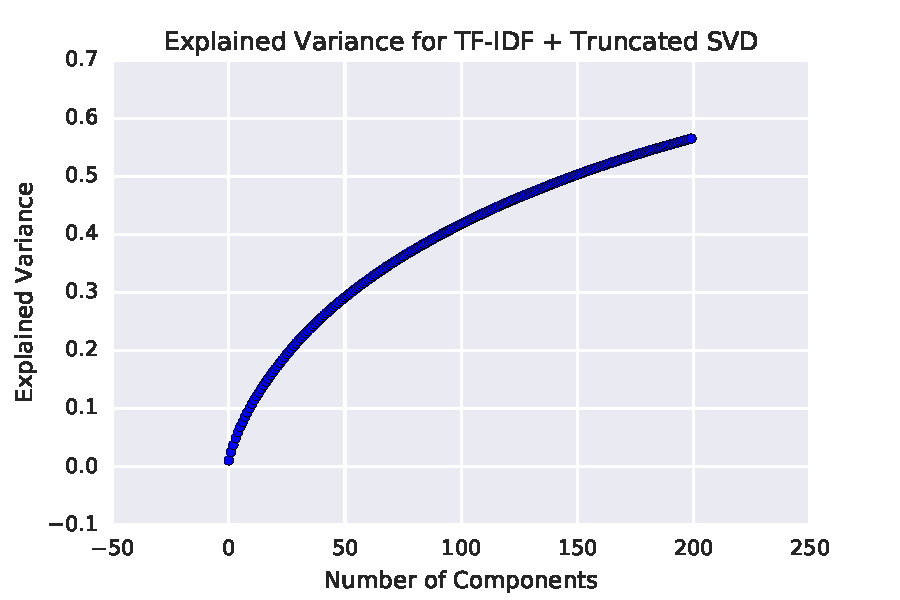
\includegraphics[width=0.55\textwidth]{variation.pdf}
  \end{multicols}

  \uncover<2->{
    \begin{center}
      \textcolor{red}{(770, 850) empty tweet vectors after tfidf for
        (training, validation) sets ($\sim$4\%)}
    \end{center}
  }
 
\end{frame}


\begin{frame}{Binary Classification}

  \begin{itemize}
  \item Six models chosen with default parameters
  \item Cross-validation  training performed with 5 folds
  \item 30\% of training samples set aside for testing
  \end{itemize}

  \uncover<2->{
    \begin{center}
      \begin{tabular}{|l|l|l|}
        \hline
        Estimator & Train Accuracy & Test Accuracy \\
        \hline
        K-Nearest Neighbors & 0.783333 & 0.792444 \\
        Logistic Regression & 0.774190 & 0.781444 \\
        SVC & 0.822619 & 0.832889 \\
        Decision Tree & 0.744524 & 0.751778 \\
        Random Forest & 0.783048 & 0.792778 \\
        Extra Trees & 0.790571 & 0.794000 \\
        \hline
      \end{tabular}
    \end{center}
  }

  \uncover<3->{
    \begin{itemize}
      \item SVC used for other statistics on validation set
    \end{itemize}

  
    \begin{center}
      \begin{tabular}{|l|l|l|l|l|}
        \hline
        Model & Accuracy & Precision & Recall & F1-Score \\
        \hline
        SVC & 0.76 & 0.90 & 0.60 & 0.72 \\
        \hline
      \end{tabular}
    \end{center}
  }

\end{frame}

\begin{frame}{Evaluating Classification Performance}
  \begin{center}
    \textcolor{blue}{\bf Performance is reasonably constant across models}
  \end{center}

  \begin{itemize}
  \item Large number of features even after truncated svd
  \item Likely reasonably linear dependence of class on features
    limits
  \item Limits probably due to remaining contamination of classes and
    low-uniqueness tweets as opposed to modeling error
  \end{itemize}

  \uncover<2->{
    \begin{center}
      \textcolor{orange}{\bf Precision is good but recall is poor}
    \end{center}

    \begin{itemize}
    \item Precision = 0.9, indicating that the identified sample of
      video game related tweets should be relatively clean, though it
      could still be overwhelmed by a large number of irrelevant
      tweets in the case of a true twitter stream
    \item Further cuts can be performed to reduce the false positives
    \item Recall is only 0.6, indicating that only 60\% video game
      related tweets in an unfiltered stream will be tagged
    \end{itemize}
  }
    


\end{frame}


\begin{frame}{ROC Curve}

  \begin{multicols}{2}
    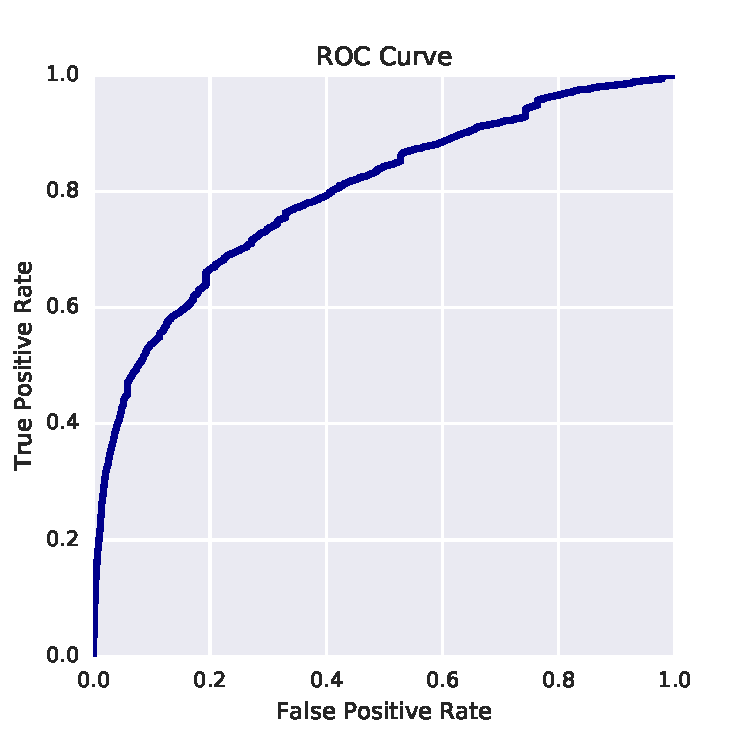
\includegraphics[width=0.55\textwidth]{ROC_Curve.pdf}

    \begin{center}
      \textcolor{red}{Total AUC = 0.79}
    \end{center}

    \begin{itemize}
    \item The model can easily be optimized for a low false rate while
      retaining a non-negligible true positive rate
    \item Achieving a high true positive rate requires acceptance of a
      significant false positive rate

    \item Consistent with intuition from precision/recall
    \end{itemize}

  \end{multicols}
\end{frame}




\begin{frame}{Refining Classification}

  \begin{multicols}{2}
    \begin{center}
      \textcolor{green}{\bf Possible Improvements}
    \end{center}

    \begin{itemize}
    \item Large sample
      \begin{itemize}
      \item Requires more processing power
      \end{itemize}
    \item Include hashtags, and possibly usernames
    \item Include emojis
    \item Prune keywords for a cleaner topic set
    \item Better balance of tweets with various keywords
    \item Apply an a-priori cut on short tweets as ``acceptable
      losses''
      \vspace*{0.5cm}
    \end{itemize}
    
    \textcolor{red}{\bf Prevalence of Keywords}
    \begin{tabular}{|l|l|l|}
      \hline
      Keyword & Percentage & Total \\
      \hline
      Zelda & 35.056 & 8764 \\
      Overwatch & 11.116 & 2779 \\
      Pokemon & 7.452 & 1863 \\
      Minecraft & 5.260 & 1315 \\
      Mario & 5.196 & 1299 \\
      Halo & 3.072 & 768 \\
      Sonic & 3.052 & 763 \\
      Mass Effect & 2.980 & 745 \\
      Resident Evil & 2.592 & 648 \\
      Call of Duty & 2.108 & 527 \\
      \hline
    \end{tabular}

  \end{multicols}

  \uncover<2->{
    \begin{center}
      \textcolor{orange}{Some coherent method of aggregating tweets may
        result in significant improvements}
    \end{center}
  }
%  \vspace*{0.5cm}
\end{frame}



\begin{frame}{Topic/Genre Modeling of Video Game Tweets}
  \begin{center}
    \textcolor{teal}{\bf Once a tweet is identified as video game
      related, it is desireable to categorize it}

    \uncover<2->{\textcolor{blue}{Two distinct methodologies}}

    \uncover<3->{
      \begin{tabular}{l|p{5cm}|p{5cm}}
        & Clustering & LDA \\
        \hline
        Use Case & Genre classification & Topic modeling \\
        \hline
        Process &
        Genres are generated by clusering the tweets, then attempt to
        identify coherent genres by prevalence of keyword labels &
        Topics are identified by performing LDA on the entire corpus
        and identifying topics based on word prevalence \\
        \hline
        Prediction &
        Identify most likely genre by comparison to LSA vector &
        Identify most likely topic through comparison to LDA
      \end{tabular}
    }
  \end{center}
 
\end{frame}

\begin{frame}{Difficulties in Genre/Topic Modeling}
  \begin{center}
    \textcolor{violet}{\bf Neither method produced meaningful initial
      results}
  \end{center}

  \begin{itemize}
  \item Clustering performed using LSA on corpus of unified tweets for
    each keyword
  \item LDA performed on original corpus of cleaned corpus
  \item Neither model yielded coherent categories
    \begin{itemize}
      \item Moreover, neither model yielded consistent categories
        using different random seets
    \end{itemize}
  \end{itemize}

  \uncover<2->{
    \begin{center}
      \textcolor{green}{\bf Too early to make conclusion on relevance
        of models vs. insufficient or insufficiently cleaned data}
    \end{center}

    \begin{itemize}
    \item Tweets from a large number of uses may simply not contain
      consistent language once keywords are removed
    \item Imbalance of classes probably damages genre clustering, and
      an iterative curation of terms may allow for meaning to be taken
      from topic modeling
    \end{itemize}
  }
\end{frame}


\begin{frame}{Conclusion}
  \begin{center}
    \textcolor{blue}{\bf Initial Binary Classification of tweets by topic
      was successful, with multiple models generating results with
      75-80\% accuracy}
  \end{center}

  \uncover<2->{
    \begin{center}
      \textcolor{green}{Many future directions may be explored}
    \end{center}

    \begin{itemize}
    \item Better cleaning and curation for improved classification
    \item More focused identification of types of tweets to be
      classified
    \item Refinement of genre/topic modeling to generate a
      sub-categorizatin procedure on tweets classified as topic
      related
    \item Application to other topics
    \item Testing using possibly-related keywords with hand-assigned
      classes (Civilization, Battlefied)
    \end{itemize}
  }
\end{frame}

%%%%%%%%%%%%%%%%%%%%%%%%%%%%%%%%%%%%%%%%%%%%%%%%%%%%%%%%%%%%%%%%%%%%%%%%%%%%%%%%

\end{document}


